\section*{PROPOSED HYBRID METHOD}\label{proposed-hybrid-method}
A hybrid method is proposed in this paper, where wave damping $B_W$
(including the speed dependent wave damping) obtained implicitly with
FNPF is used together with the viscous damping contributions from
Ikeda's method. The viscous damping is added to the FNPF simulations by
injecting the viscous parts of the linear and quadratic damping
coefficients (obtained with Ikeda's method) to the equation of motion.
Ikeda's method divides roll damping into five damping components so that
the total damping can be calculated as \citep{7505983/937PN5DT},
\begin{equation}
B = B_F + B_E + B_L + B_W + B_{BK}
\end{equation}
Where $B_F$ is the skin friction component, $B_E$ is the eddy
generation component, $B_L$ is hull lift component, $B_W$ is roll
wave generation component and $B_{BK}$ is the bilge keel component.
Ikeda's method propose semi empirical formulas for the viscous damping
components: $B_F$, $B_E$, $B_{BK}$ and $B_L$ so that viscous
damping can be obtained from,
\begin{equation}
\label{eq:viscous_damping}
B_{visc} = B_F + B_E + B_L
\end{equation}
\quad In order to reduce the number of uncertain parameters, the bilge
keel damping $B_{BK}$ has been exluded in
Eq.\ref{eq:viscous_damping}, thereby assuming that the ship does
not have any bilge keels.
\quad The skin friction damping $B_F$ is calculated using
\citep{7505983/CKCMI3N9} which is implementation according to the
description in \citep{7505983/UGK6YEVD}. The scale effects of roll
damping are considered to mainly be associated with the skin friction
component $B_F$ \citep{7505983/FB64RGPF}. This component constitute a
very small part of the total damping for the full scale ship, but a
substantial part for the model scale ship used in this study. This is
therefore the only component in Ikedas method that needs to be
recalculated when the scale changes.
\quad The hull lift damping $B_L$ is calculated according to
\citep{7505983/937PN5DT} and implemented as described in
\citep{7505983/UYUAYY7E} where the calculations have been improved with a
linear interpolation of the values for $\kappa$ from
\citep{7505983/937PN5DT}.
\quad Ikeda's method calculates the roll damping at a certain roll angle
frequency $\omega$ and roll angle amplitude $\phi_a$. A schematic
graph of how the parameters vary with speed and roll angle amplitude
$\phi_a$ is shown in Fig.\ref{fig:ikeda_generic}. In this
figure, roll amplitude is first varied at zero speed (left). The speed
is then varied at constant roll angle amplitude of 10 degrees (middle).
The amplitude is then gradually reduced at the highest speed down to
zero again (right).
\quad Assumming that the trends are correct in Ikeda's method it can be
noted from the amplitude variations at zero knots (left):
\begin{itemize}
\item $B_W$ does not change with amplitude, implying that they only contribute to the linear part ($B_1$) of the damping. (The $B_W$ was calculated with strip theory here)
\item $B_F$ has a small amplitude dependancy but the linear part is dominating.
\item $B_E$ has a large amplitude depandancy and only contributes to the quadratic damping ($B_2$)\citep{7505983/4AFVVGNT}.
\end{itemize}
\quad Looking at the speed variation (middle):
\begin{itemize}
\item At low speed $B_F$ and $B_E$ are the dominating components. (Note that this ship does not have bilge keels, as that would otherwise also be a large component).
\item At high speed the $B_E$ has almost disappeared and is replaced by the $B_L$ which is now the dominating component.
\item $B_F$ has a large contribution for all speeds (at model scale).
\end{itemize}
\quad Looking at the roll amplitude variation (right):
\begin{itemize}
\item (Please note that this x-axis is revered in this graph)
\item $B_L$ does not change with amplitude, implying that they only contribute to the linear part ($B_1$) of the damping.
\item $B_F$ has a small amplitude dependancy but the linear part is dominating.
\end{itemize}
\begin{figure}[H]
\begin{center}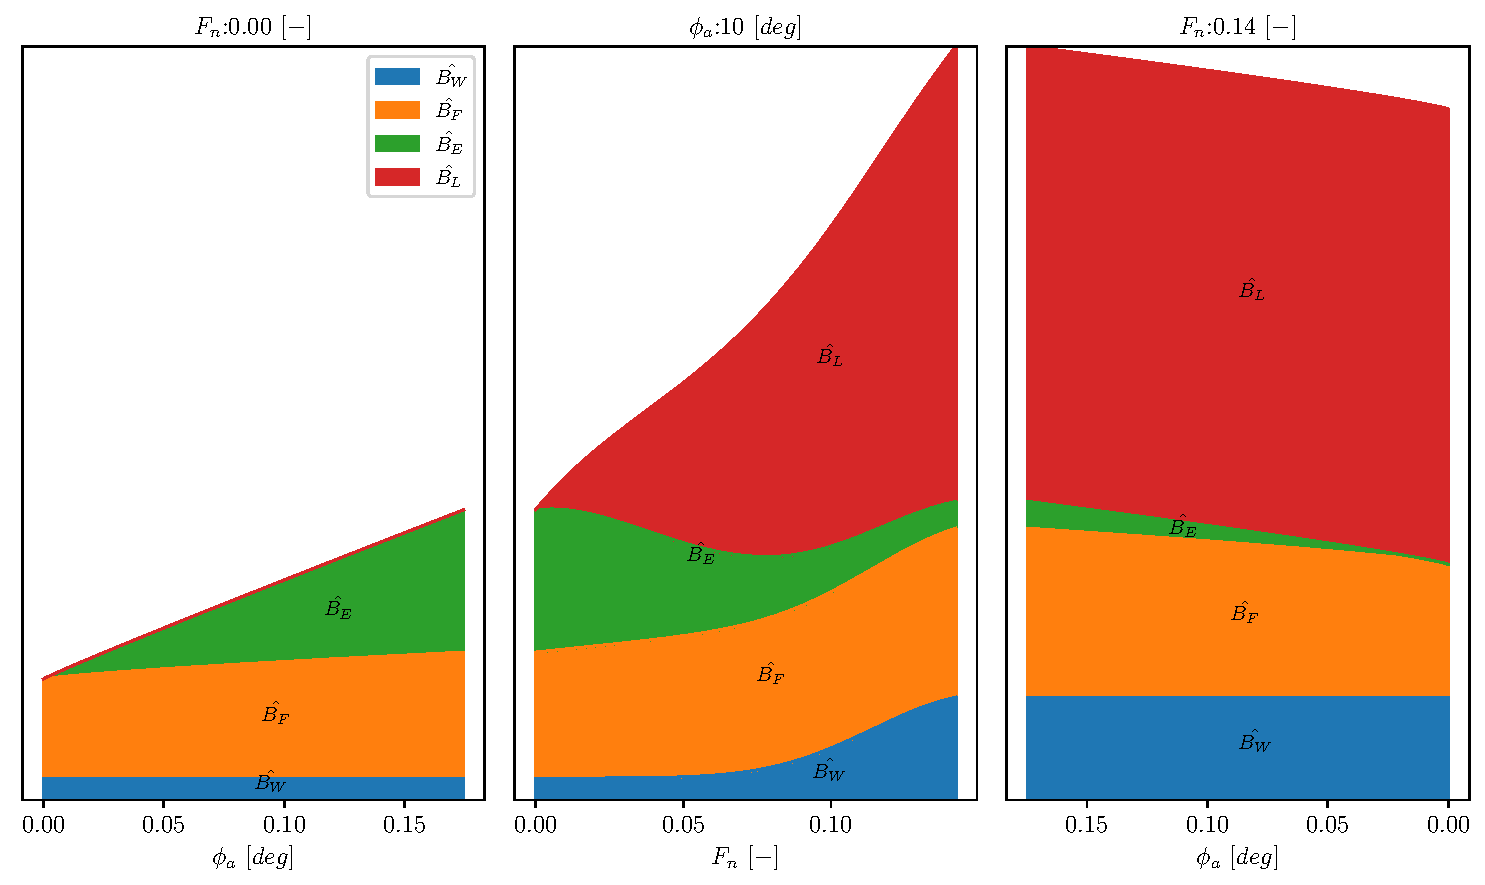
\includegraphics[width = 0.5\textwidth]{figures/ikeda_generic.pdf}\end{center}
\vspace{-1cm}
\caption{Example of roll damping predicted with Ikeda's method}
\label{fig:ikeda_generic}
\end{figure}
When the damping predicted with Ikeda's method was compared with
corresponding model tests (see section "\nameref{se:validation}"), it
was found that the results were in poor agreement for the zero speed
case (see Fig.\ref{fig:ikeda} (left)) but quite good results at
speed. This was pointing towards the eddy damping being incorrect in the
current implementation of Ikeda's method. A thorough investigation of
the eddy damping prediction was therefore conducted which is described
in the next section.
\subsection*{Eddy damping}\label{eddy-damping}
At zero speed, the eddy damping $B_E$ represents a nonlinear force
caused by the two-dimensional separation near the bilge keel. The eddy
damping is also nonlinear at speed where it represents the nonlinear
part part of the hydrodynamic lift damping ($B_L$ represents the
linear part). The speed dependancy of the eddy damping is calculated
using the following semi empirical formula \citep{7505983/937PN5DT}:
\begin{equation}
\frac{B_{E}}{B_{E0}} = \frac{0.0016 K^{2}}{0.0016 K^{2} + 1}
\label{eq:eddy_speed}
\end{equation}
Where $K$ is the reduced frequency:
\begin{equation}
K = \frac{L_{pp} \omega}{V}
\label{eq:K}
\end{equation}
For the zero speed case, Fig.\ref{fig:eddy_sigma} is an
illustration of how the eddy damping changes with bilge radius as
predicted with the current implementation of the method. It seems that
the damping approaches zero very fast as the bilge radius increases.
Having just a small rounding of the bilge, compared to a square section,
will thereby have a great impact on the eddy roll damping.
\begin{figure}[H]
\begin{center}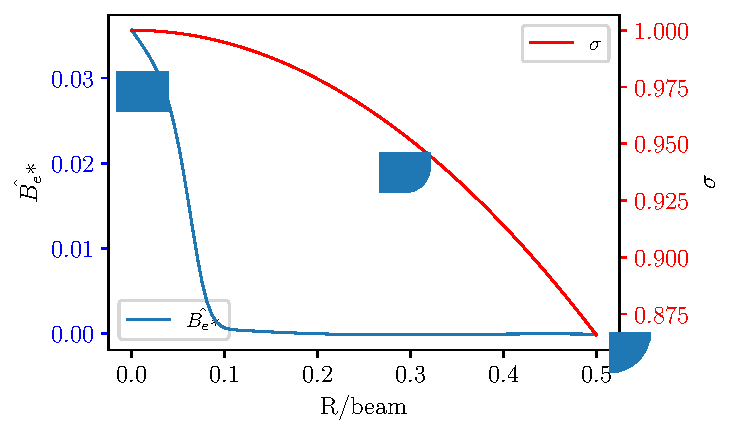
\includegraphics[width = 0.5\textwidth]{figures/eddy_sigma.pdf}\end{center}
\vspace{-1cm}
\caption{Sectional eddy damping (left y-axis) and $\sigma$ (right y-axis) vs. bilge radius (x-axis).}
\label{fig:eddy_sigma}
\end{figure}
The eddy damping prediction at zero speed is based on a regression
formula from experiements on a number of two-dimensional cylinders with
various sections \citep{7505983/4AFVVGNT}. The eddy damping per unit
length of these sections can be expressed as:
\begin{equation}
B'_{E0} = \frac{4 C_{r} T_{s}^{4} \omega \phi_{a} \rho}{3 \pi}
\label{eq:eddy_section}
\end{equation}
The total eddy damping can be obtained as an integral over the sections
along the ship hull:
\begin{equation}
B_{E0} = \int\limits_{AP}^{FP} B'_{E0}\, dx_{s}
\label{eq:eddy_integration}
\end{equation}
It can be seen from the section damping
(Eq.\ref{eq:eddy_section}) that the eddy damping increases
linearly with both roll amplitude and frequency, and that it will go to
zero for small amplitudes and frequencies. This means that eddy damping
is only included in the quadratic damping term ($B_2$). The $C_r$
coefficient in (Eq.\ref{eq:eddy_section}) is assumed to be
entirely depending on the hull form and is calculated using the
regression formula in \citep{7505983/4AFVVGNT}. This regression formula
is based on: section area coefficient $\sigma$ and the Lewis section
coefficients: $a_1$ and $a_3$. An alternative regression formula for
$C_r$ has however been developed for this paper, as described below.
This regression is based the same experimental results
\citep{7505983/4AFVVGNT}, collected by the authors using manual
digitalization \citep{7505983/8YUE24LM}.
The nondimensional damping taken from \citep{7505983/4AFVVGNT} is
expressed using an asterisk, or star symbol (*), to emphase that this
component only has a quadratic part of the damping. This stared damping
is defined as:
\begin{equation}
\hat{B}_{E0} = \frac{8 \hat{B^*}_{E}}{3 \pi}
\label{eq:B_E_star_hat}
\end{equation}
$\hat{B_E^*}$ and $(B_W+B_F)^*$ are the experimental values taken
from \citep{7505983/4AFVVGNT}. Which add up to the total damping:
\begin{equation}
\hat{B^*} = \hat{B^*}_{E} + \hat{B^*}_{F} + \hat{B^*}_{W}
\label{eq:B_star_hat}
\end{equation}
And the $C_r$ can be calculated from the experiments as:
\begin{equation}
C_{r} = \frac{3 \pi B_{s} \hat{B}_{E0} beam^{2} \sigma}{4 T_{s}^{3} \hat{\omega} \phi_{a}}
\label{eq:C_r_2}
\end{equation}
A simple decision tree model is used for the $C_r$ regression, based
on the same Lewis section coefficients from the regular regression
formula. The fitted decision tree is illustrated in
Fig.\ref{fig:decision_tree}.
\begin{figure}[H]
\begin{center}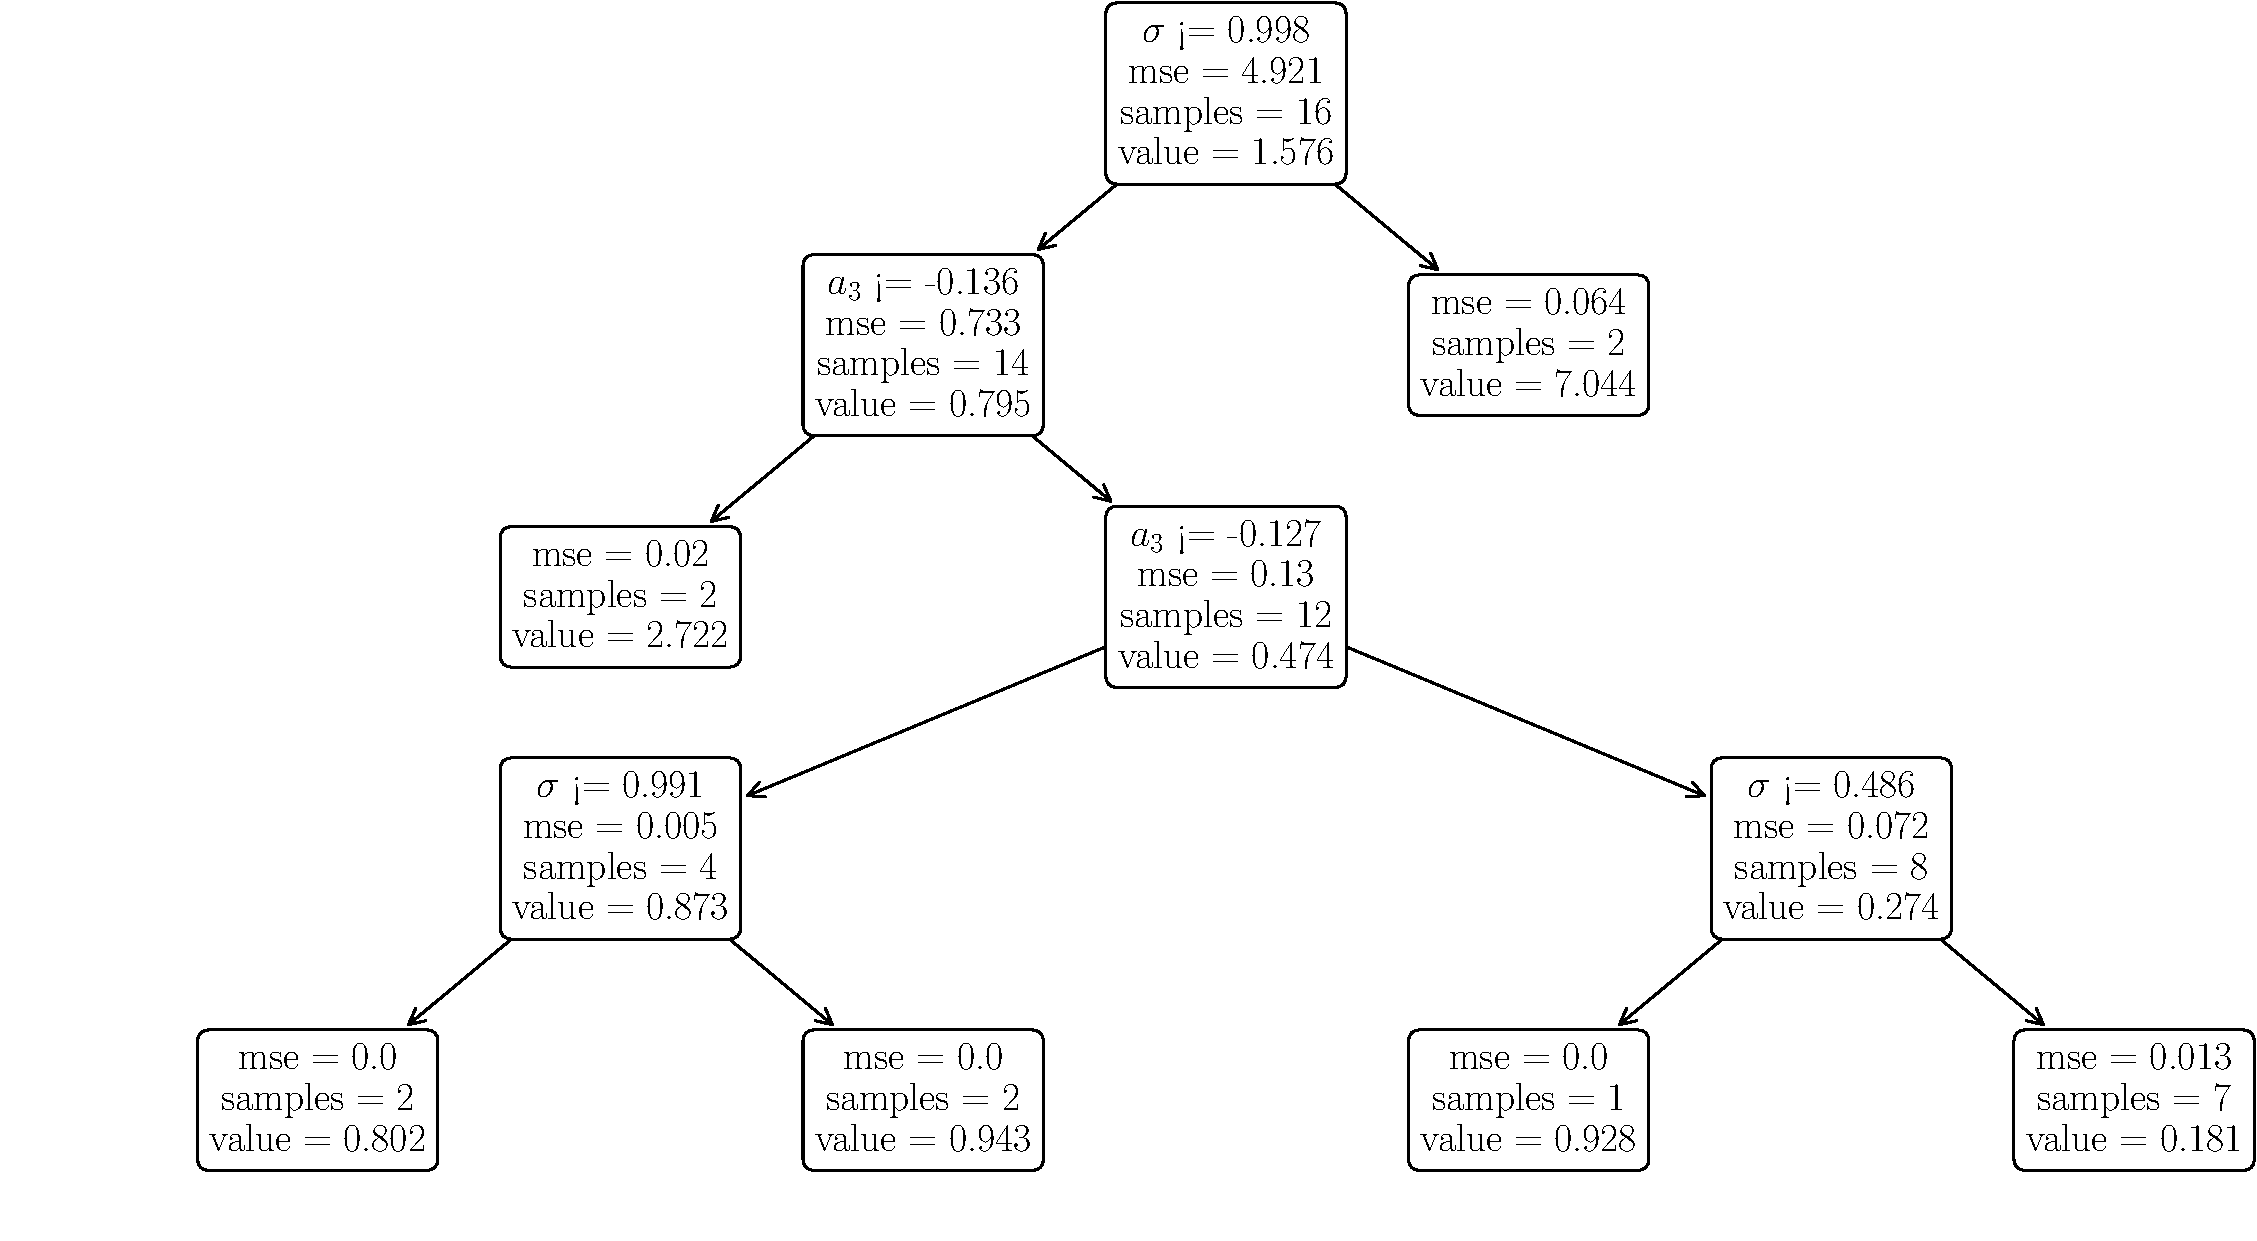
\includegraphics[width = 0.5\textwidth]{figures/decision_tree.pdf}\end{center}
\vspace{-1cm}
\caption{Decision tree to predict $C_r$}
\label{fig:decision_tree}
\end{figure}
Even though this tree is very simple it has very good accuracy in
reproducing the results from Ikedas experiments ($r^2=0.996$) compared
to ($r^2=0.762$) when using Ikeda's method.
Fig.\ref{fig:ikeda_sections} shows $C_r$ from the experiments
and corresponding predictions with Ikeda's method and the decision tree.
The capital letters refer to cylinder sections from the experiments
\citep{7505983/4AFVVGNT}.
\begin{figure}[H]
\begin{center}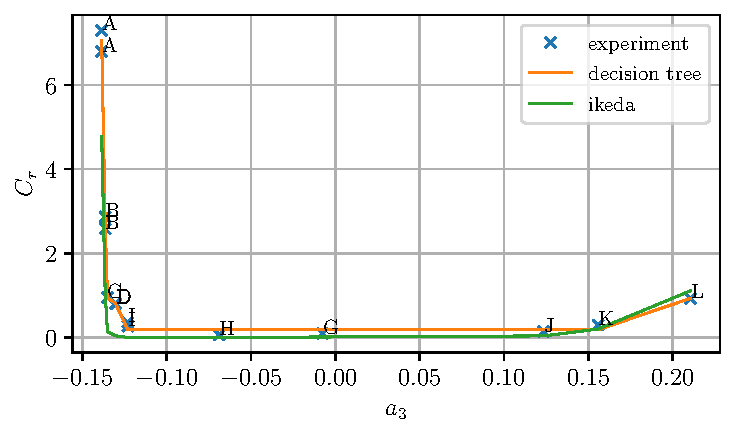
\includegraphics[width = 0.5\textwidth]{figures/ikeda_sections.pdf}\end{center}
\vspace{-1cm}
\caption{$C_r$ for cylinder sections from experiments and predicted with Ikeda's method and the decision tree model.}
\label{fig:ikeda_sections}
\end{figure}
\subsection*{FNPF method}\label{fnpf-method}
\label{fnpf-method} The wave damping was obtained using parameter an
identification technique, as described in section: "\nameref{se:pit}",
on roll decay simulation using the fully nonlinear potential flow
method. This method is characterized by the application of the complete
dynamic and kinematic free surface boundary conditions on the
instantaneous free surface as well as the body-exact approach where the
instantaneous wetted body surface is considered in the boundary value
problem for the velocity potential, i.e. no linearizations are made to
the governing equations of the potential flow problem.
\quad The method used in this study employs a boundary element method
(BEM) \citep{7505983/FD4N3DW2} to solve the boundary value problem for
the velocity potential.
\quad The free surface boundary conditions and the motions of the
floating body introduce time dependency to the boundary value problem.
The BEM is coupled with the mixed Eulerian-Lagrangian method (MEL)
\citep{7505983/ZKB494GT} which is used for the evolution of free surface.
A fourth-order Adams-Bashforth-Moulton time integral scheme is then used
to evolve free surface and the rigid-body body motions in time.
\quad The benefit with the FNPF method is the lack of linearizations to
the free surface potential flow where all interactions between the
undisturbed incident flow and surface piercing body is captured
implicitly in the total velocity potential, including inviscid (wave)
damping due to radiation and diffraction. The downside is the larger
computational cost compared to many other potential flow based methods
due to the fact that a boundary value problem for the velocity potential
must be solved at least once every time step, depending on the specifics
of the time integral scheme. However, FNPF methods are still typically
less computationally demanding than for example URANS methods, making
them attractive choices for seakeeping problems.
